\chapter{Conclusions and Future Work}

In this project a complete platform has been developed and its value has been demonstrated by
testing it with real users and by developing two services using the platform. In this section the
conclusions of this development are presented, preceded with the usage statistics of the project,
one of the objectives of the project itself.

\section{Usage Statistics}

This project was tested during the Deusto's ForoTech engineering week (figure~\ref{fig:forotech}).
During that testing that lasted for 8 days, hundreds of students saw the system. There was a live
demo in the forum itself, where students learned how to play the game and received their own user
and password to play from home. During those demonstrations, the experiment was used 72 times, with
a total of 16,119.5 seconds of use (about 4 hours and a half).

\begin{figure}[ht]
	\centering
	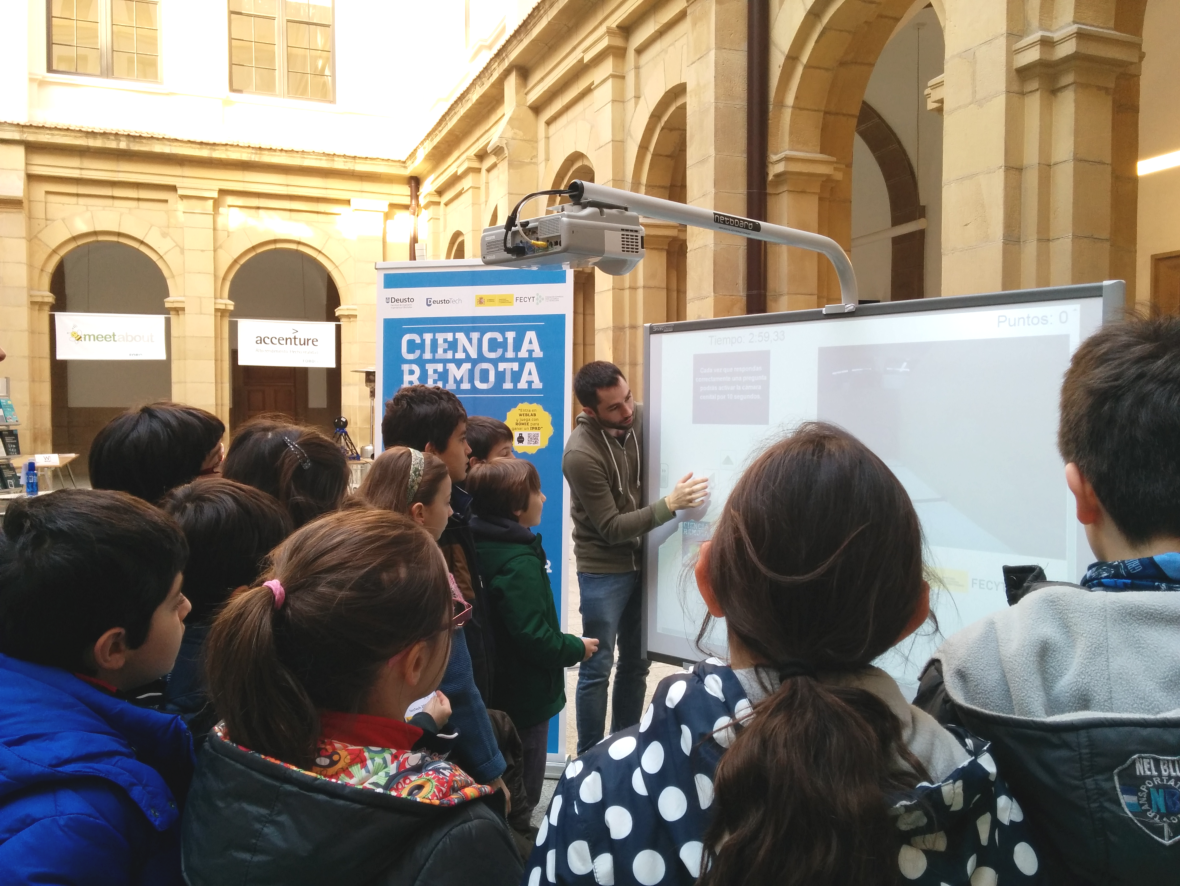
\includegraphics[height=0.3\textheight]{fig/forotech.jpg}
	\caption{Students looking at the ForoTech demonstration.}
	\label{fig:forotech}
\end{figure}

Moreover, 64 users logged in and played from home, with a total of 665 uses (more than 10 times per
user) with a total of 145,155.22 seconds of use (about 40 hours and 19 minutes), which is about
2,268 seconds per user or about 38 minutes.

The average game was of about 200 seconds (about 3 minutes and 20 seconds) and the day with most
uses was the Wednesday (the first day of use) in the afternoon, where the system had 164 uses. There
were no important issues with the robot, and most of them were hardware related, due to failing
pieces that were changed rapidly.

The final top five ranking of the competition was the one in table~\ref{tab:ranking}. The first two
received an iPad (figure~\ref{fig:prizes}). There was a real competition where users were playing
until the last second of the competition, literally.

\begin{table}[ht]
	\centering
	\caption{Romie competition's top five ranking.}\label{tab:ranking}
	\begin{tabular}{cc}
		\toprule
		\textbf{Name} & \textbf{Points} \\
		\midrule
		Telmo		& 6,917,714	\\
		Hodei		& 6,915,484	\\
		Joshua		& 728,968	\\
		Martin		& 700,010	\\
		Adair		& 589,400	\\
		\bottomrule
	\end{tabular}
\end{table}

\begin{figure}[ht]
	\centering
	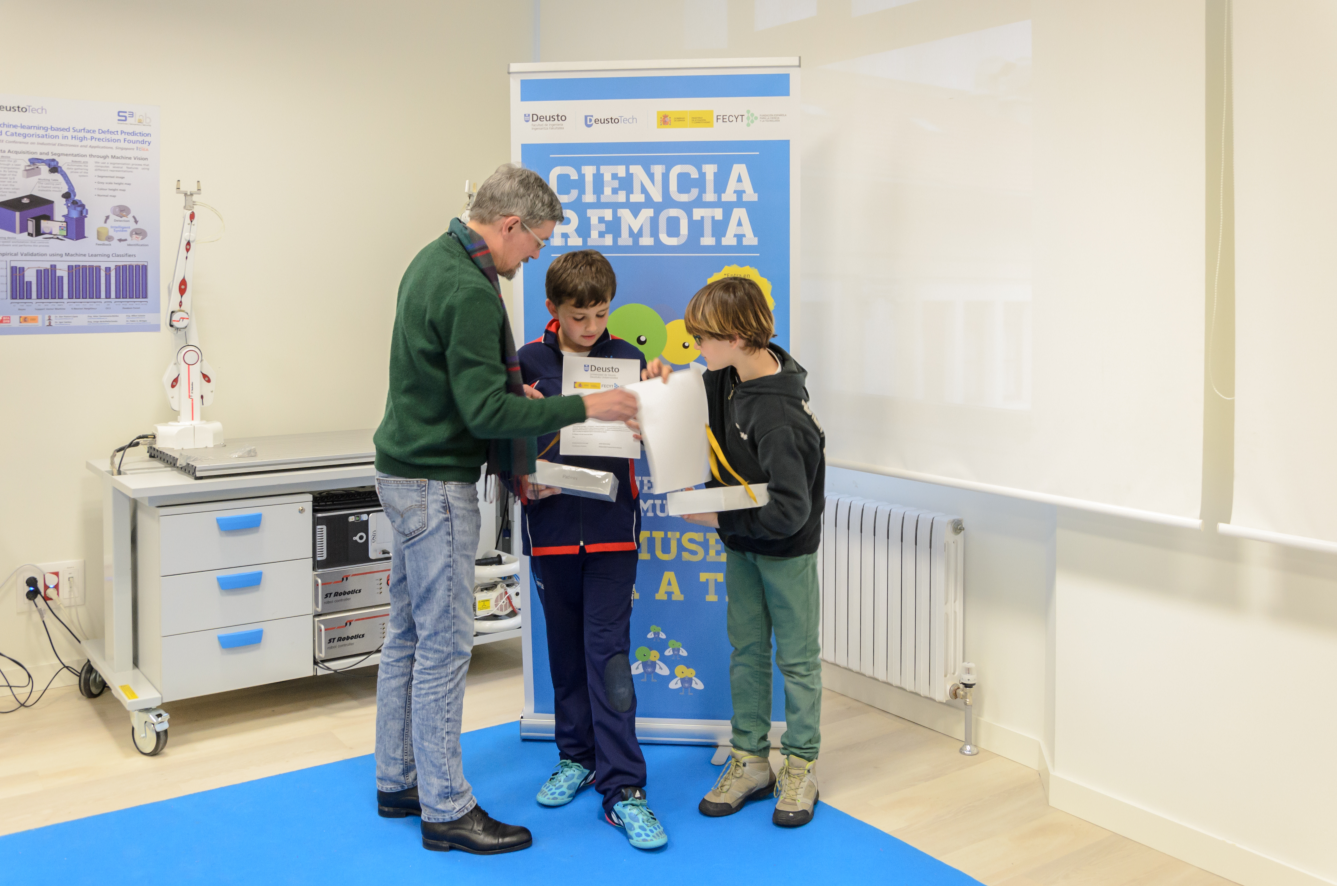
\includegraphics[height=0.3\textheight]{fig/prizes.jpg}
	\caption{Telmo and Hodei receiving the prize for wining the competition sponsored by \acrshort{fecyt}.}
	\label{fig:prizes}
\end{figure}

\section{Conclusions}

As it can be seen, the project has ended successfully, since it has fulfilled all the objectives
proposed at the beginning of it. The challenges have been difficult to complete but with hard work,
all of them have been successfully accomplished.

The main outcomes for the platform have been that this project has a big potential. As it has been
demonstrated, it is easy to use, as it has been seen, since 64 users were able to play with it. This
fulfills the requirements of usability.

It has been integrated in the WebLab-Deusto platform, as the objectives demanded, which will allow
further use of the platform once the schools integrate it with their current use of WebLab-Deusto.

It has received a petition that will be made real for the end of 2015 of installing the game in
the Domus museum in A Coruña, Spain, under the ``Ciencia remota'' project of the \acrshort{fecyt}.
This fulfills the objective of disseminating the platform.

The two main environments of the platform have been developed and are fully functional. The game has
been tested with dozens of uses, while the visual programming \acrshort{ide} has shown great
potential on programming the robot with full control of the execution.

The usage statistics seen in the previous section were part of the objectives and show how the real
use of the platform has been. It has been demonstrated the reliability of both the software and the
hardware of the platform as well as the viability for heavy load situations. In overall, the project
has demonstrated that it can be deployed in production, like it has been done in WebLab-Deusto.

\section{Future Lines of Work}

The current work is a complete system with its game modes. In WebLab-Deusto it is currently deployed
in production, so it can be considered finished. Nevertheless, there are many ways to improve both
the user experience and the results of this project. For instance, here are a few that could be
developed in future research:

\begin{itemize}

	\item \textbf{Augmented reality}: The experiment could be equipped with augmented reality to
	give more interactivity to the user. It could show any sort of 3D game information in the
	labyrinth. Some scenarios have been suggested, such as a game where the user would have to
	recover virtual elements from the labyrinth moving across all of it and use them to build
	virtual hardware. The possibilities are unlimited.

	\item \textbf{Computer vision}: Computer vision could be added to both top and on-board cameras.
	This way, the user and the software developed could have more information about the position of
	the robot or even about information in the labyrinth.

	It could help putting \acrshort{qr}  (\acrlong{qr}) codes in the walls to show something to the
	user. Moreover, top camera's computer vision could be used to locate the robot and try to
	challenge the user to move to a concrete place.

	\item \textbf{New game modes}: The platform currently provides a trivial type game, to which a
	psychological experiment can be added through configuration (is not enabled by default) and a
	visual programming \acrshort{ide}, where the user can program the robot. Nevertheless, these are
	only examples of the potential of this project.

	The platform is prepared, thanks to its modular \acrshort{api}s to host more experiments and
	games that could use it. It could be used for teaching, for experimenting with art (painting the
	walls or asking the user to paint patterns with the robot movement) or for any other use the
	imagination can lead to.

	\item \textbf{Internationalization}: Currently the platform is only provided in Spanish. It
	would be great to add a \acrlong{i18n} or \acrshort{i18n} \acrshort{api} to be able to provide
	it in more languages.

\end{itemize}

In any case, the current platform is extensible enough to allow any kind of experiment being
developed, always thinking on the current hardware. And, as it has been seen before, there is
already a plan to deploy the game in the Domus museum in A Coruña, Spain. This way, the big
potential of the project is demonstrated, as well as its future lines of work, that can lead it to
be used in many scopes.
